\lab{Pandas IV: Time Series}{Pandas IV: Time Series}
\objective{Learn how to manipulate and prepare time series in pandas in preparation for analysis}
\label{lab:pandas4}


\section*{Introduction: What is time series data?}
Time series data is ubiquitous in the real world. Time series data is any form of data that comes attached to a timestamp (i.e. Sept 28, 2016 20:32:24) or a period of time (i.e. Q3 2012). Some examples of time series data include:
\begin{itemize}
    \item stock market data
    \item ocean tide levels
    \item number of sales over a period of time
    \item website traffic
    \item concentrations of a certain compound in a solution over time
    \item audio signals
    \item seismograph data
    \item and more...
\end{itemize}

Notice that a common feature of all these types of data is that the values can be tied to a specific time or period of time.

In this lab, we will not go into depth on the analysis of such data. Rather, we will discuss some of the tools provided in pandas for cleaning and preparing time series data for further analysis.

\section*{Initializing Time Series in $\texttt{pandas}$}
To take advantage of all the time series tools available to us in pandas, we need to make a few adjustments to our normal DataFrame.

\subsection*{The $\texttt{datetime}$ Module and Initializing a $\texttt{DatetimeIndex}$}
For pandas to know to treat a DataFrame or Series object as time series data, the index must be a \li{DatetimeIndex}. pandas utilizes the \li{datetime.datetime} object from the \li{datetime} module to standardize the format in which dates or timestamps are represented.

\begin{lstlisting}
>>> from datetime import datetime

>>> datetime(2016, 9, 28) # 9/28/2016
datetime.datetime(2016,9,28,0,0)

>>> datetime(2016, 9, 28, 21, 12, 48) # 9/28/2016 9:12:48 PM
datetime.datetime(2016, 9, 28, 21, 12, 48)
\end{lstlisting}

Unsurprisingly, the format for dates varies greatly from dataset to dataset. The \li{datetime} module comes with a string parser (\li{datetime.strptime()}) flexible enough to translate nearly any format into a \li{datetime.datetime} object. This method accepts the string representation of the date, and a string representing the format of the string. See Table \ref{table:date_formats} for all the options.

\begin{table}[h!]
\begin{center}
    \begin{tabular}{|c|l|}
        \hline
        \li{\%Y} & 4-digit year \\
        \li{\%y} & 2-digit year \\
        \li{\%m} & 2-digit month \\
        \li{\%d} & 2-digit day \\
        \li{\%H} & Hour (24-hour) \\
        \li{\%I} & Hour (12-hour) \\
        \li{\%M} & 2-digit minute \\
        \li{\%S} & 2-digit second \\
        \hline
    \end{tabular}
\end{center}
\caption{Formats recognized by \li{datetime.strptime()}}
\label{table:date_formats}
\end{table}

Here are some examples of using \li{datetime.strptime()} to parse the same date from different formats.
\begin{lstlisting}
>>> datetime.strptime("2016-9-28", "%Y-%m-%d")
datetime.datetime(2016, 9, 2, 0, 0)

>>> datetime.strptime("9/28/16", "%m/%d/%y")
datetime.datetime(2016, 9, 2, 0, 0)

>>> datetime.strptime("2016-9-28 9:12:48", "%Y-%m-%d %I:%M:%S")
datetime.datetime(2016, 9, 28, 9, 12, 48)
\end{lstlisting}

If the dates are in an easily parsible format, pandas has a method \li{pd.to_datetime()} that can turn a whole pandas \li{Series} into \li{datetime.datetime} objects. In the case of the index, the index is automatically converted to a \li{DatetimeIndex}. This index type is what distinguishes a regular \li{Series} or \li{DataFrame} from a time series.

\begin{lstlisting}
>>> dates = ["2010-1-1", "2010-2-1", "2010-3-1", "2011-1-1",
... "2012-1-1", "2012-1-2", "2012-1-3"]
>>> values = np.random.randn(7,2)
>>> df = pd.DataFrame(values, index=dates)
>>> df
                 0         1
2010-1-1  0.566694  1.093125
2010-2-1 -0.219856  0.852917
2010-3-1  1.511347 -1.324036
2011-1-1  0.300766  0.934895
2012-1-1  0.212141  0.859555
2012-1-2  1.483123 -0.520873
2012-1-3  1.436843  0.596143

>>> df.index = pd.to_datetime(df.index)
\end{lstlisting}

\begin{info}
In earlier versions of pandas, there was a dedicated TimeSeries data type. This has since been depricated, however the functionality remains. Therefore, if you happen to read any materials that reference the TimeSeries data type, know that the cooresponding functionality is likely still in place as long as you have a \li{DatetimeIndex} associated with your Series or DataFrame.
\end{info}

\begin{problem} \label{prob:DJIA}
The provided dataset, ``DJIA.csv" is the daily closing value of the Dow Jones Industrial Average for every day over the past 10 years. Read this dataset into a Series with a DatetimeIndex. Replace any missing values with \li{np.nan}. Lastly, cast all the values in the Series to floats. We will use this dataset for many problems in this lab.
\end{problem}

\section*{Handling Data Without Marked Timestamps}

There will be times you will need to analyze time series data that does not come marked with an index. For example, you may have the a list of bank account balances at the beginning of every month for the last 5 years. You may have heart rate readings every 10 minutes for the past week. pandas provides efficient tools for generating indices for these kinds of siutations.

\subsection*{The $\texttt{pd.date\_range()}$ Method}

The \li{pd.date\_range()} method is analogous to \li{np.arange()}. The parameters we will use most are described in Table \ref{table:date_params}.

\begin{table}[h!]
\begin{center}
    \begin{tabular}{|r|l|}
        \hline
        \li{start} & start of date range \\
        \li{end} & end of date range \\
        \li{periods} & the number of dates to include in the date range \\
        \li{freq} & the amount of time between dates (similar to ``step") \\
        \li{normalize} & trim the time of the date to midnight \\
        \hline
    \end{tabular}
\end{center}
\caption{Parameters for \li{datetime.strptime()}}
\label{table:date_params}
\end{table}

Exactly two of the parameters \li{start}, \li{end}, and \li{periods} must be defined to generate a range of dates. The \li{freqs} parameter accepts a variety of string representations. The accepted strings are referred to as \emph{offset aliases} in the documentation. See Table \ref{table:range_freqs} for a sampling of some of the options. For a complete list of the options, see \url{http://pandas.pydata.org/pandas-docs/stable/timeseries.html#offset-aliases}.

\begin{table}[h!]
\begin{center}
    \begin{tabular}{|r|l|}
        \hline
        \li{D} & calendar daily (default) \\
        \li{B} & business daily \\
        \li{H} & hourly \\
        \li{T} & minutely \\
        \li{S} & secondly \\
        \li{MS} & first day of the month \\
        \li{BMS} & first weekday of the month \\
        \li{W-MON} & every Monday \\
        \li{WOM-3FRI} & every 3rd Friday of the month \\
        \hline
    \end{tabular}
\end{center}
\caption{Parameters for \li{datetime.strptime()}}
\label{table:range_freqs}
\end{table}

\begin{lstlisting}
>>> pd.date_range(start='9/28/2016 16:00', periods=5)
DatetimeIndex(['2016-09-28 16:00:00', '2016-09-29 16:00:00',
               '2016-09-30 16:00:00', '2016-10-01 16:00:00',
               '2016-10-02 16:00:00'],
              dtype='datetime64[ns]', freq='D')

>>> pd.date_range(start='1/1/2016', end='1/1/2017', freq="2BMS" )
DatetimeIndex(['2016-01-01', '2016-03-01', '2016-05-02', '2016-07-01',
               '2016-09-01', '2016-11-01'],
              dtype='datetime64[ns]', freq='2BMS')


>>> pd.date_range(start='9/28/2016 16:00',
            end='9/29/2016 16:30', freq="10T")
DatetimeIndex(['2016-09-28 16:00:00', '2016-09-28 16:10:00',
               '2016-09-28 16:20:00', '2016-09-28 16:30:00'],
              dtype='datetime64[ns]', freq='10T')
\end{lstlisting}

The \li{freq} parameter also supports more flexible string representations.
\begin{lstlisting}
>>> pd.date_range(start='9/28/2016 16:30', periods=5, freq="2h30min")
DatetimeIndex(['2016-09-28 16:30:00', '2016-09-28 19:00:00',
               '2016-09-28 21:30:00', '2016-09-29 00:00:00',
               '2016-09-29 02:30:00'],
              dtype='datetime64[ns]', freq='150T')
\end{lstlisting}

\begin{problem}
The ``paychecks.csv" dataset has values of an hourly employee's last 93 paychecks. He started working March 13, 2008. This company hands out paychecks on the first and third Fridays of the month. However, ``paychecks.csv" is not indexed explicitly as such. To be able to manipulate it as a time series in pandas, we will need to add a \li{DatetimeIndex} to it. Read in the data and use \li{pd.date\_range()} to generate the \li{DatetimeIndex}.

Hint: to combine two \li{DatetimeIndex} objects, you can use the \li{.union()} method of \li{DatetimeIndex} objects.
\end{problem}

\section*{Plotting Time Series}
The process for plotting a time series is identical to plotting any other Series or DataFrame. For more information and examples, refer back to Lab \ref{lab:pandas2}.

\begin{problem} \label{prob:plot}
Plot the DJIA dataset that you read in as part of Problem \ref{prob:DJIA}. Label your axes and title the plot.
\end{problem}

\section*{Dealing with Periods Instead of Timestamps}
It is often important to distinguish whether a given figure corresponds to a single point in time or to a whole month, quater, year, decade, etc. A \li{Period} object is better suited for the summary over a \emph{period} of time rather than the timestamp of a specific event.

Some example of time series that would merit the use of periods would include,
\begin{itemize}
    \item The number of steps a given person walks in a day.
    \item The box office results per week for a summer blockbuster.
    \item The population changes of a given city per year.
    \item etc.
\end{itemize}

\subsection*{The $\texttt{Period}$ Object}
The principle parameters of the \li{Period} are \li{"value"} and \li{"freq"}. The \li{"value"} paramter indicates the label for a given \li{Period}. This label is tied to the \emph{end} of the defined \li{Period}. The \li{"freq"} indicates the length of the \li{Period} and also (in some cases) indicates the offset of the \li{Period}. The \li{"freq"} parameter accepts the majority, but not all, of frequencies listed in Table \ref{table:range_freqs}.

These nuances are best clarified through examples.

\begin{lstlisting}
# The default value for `freq' is "M" meaning month.
>>> p1 = pd.Period("2016-10")
>>> p1.start_time
Timestamp('2016-10-01 00:00:00')

>>> p1.end_time
Timestamp('2016-10-31 23:59:59.999999999')

# A `freq' value of 'A-DEC' indicates a annual period
#    with the end of the period occuring in December.
>>> p2 = pd.Period("2016-10-03", freq="A-DEC")
>>> p2.start_time
Timestamp('2007-01-01 00:00:00')

>>> p2.end_time
Timestamp('2007-12-31 23:59:59.999999999')

# Notice that the Period object that is created is the
#   week of the year when the given date occurs. Also
#   note that "W-SAT" indicates we wish to treat
#   Saturday as the last day of the week (and therefore
#   Sunday as the first day of the week.)
>>> p3 = pd.Period("2016-10-03", freq="W-SAT")
>>> p3
Period('2016-10-02/2016-10-08', 'W-SAT')
\end{lstlisting}

\subsection*{The $\texttt{pd.period\_range()}$ Method}
Like the \li{pd.date\_range()} method, the \li{pd.period\_range()} method is useful for generating a \li{PeriodIndex} for unindexed data. The syntax is essentially identical to that of \li{pd.date\_range()}. When using \li{pd.period\_range()}, remember that the \li{"freq"} parameter marks the end of the period.

\begin{lstlisting}
# a 'freq' value of 'Q-DEC' means that Q4 ends in December.
>>> pd.period_range("2008", "2010-12", freq="Q-DEC")
PeriodIndex(['2009Q1', '2009Q2', '2009Q3', '2009Q4', '2010Q1', '2010Q2',
             '2010Q3', '2010Q4'], dtype='int64', freq='Q-DEC')
\end{lstlisting}

\subsection*{Other Useful Functionality and Methods}
After creating a \li{PeriodIndex}, you have the option to redefine the \li{"freq"} parameter using the \li{asfreq()} method.

\begin{lstlisting}
>>> p = pd.period_range("2010-03", "2011", freq="3M")
PeriodIndex(['2010-03', '2010-06', '2010-09', '2010-12'],
            dtype='int64', freq='3M')

# Change frequency to be "Q-DEC" instead of "3M"
>>> p = p.asfreq("Q-DEC")
>>> p
PeriodIndex(['2010Q2', '2010Q3', '2010Q4', '2011Q1'],
            dtype='int64', freq='Q-DEC')
\end{lstlisting}

Say you have created a \li{PeriodIndex}, but the bounds are not exactly where you expected they would be. You can actually shift \li{PeriodIndex} obejcts by adding or subtracting an integer, $n$. The resulting \li{PeriodIndex} will be shifted by $n$ $\times$ \li{freq}.

\begin{lstlisting}
# Shift index by 1
>>> p -= 1
>>> p
PeriodIndex(['2010Q1', '2010Q2', '2010Q3', '2010Q4'],
            dtype='int64', freq='Q-DEC')
\end{lstlisting}

If for any reason you need to switch from periods to timestamps, pandas provides a very simple method to do so.

\begin{lstlisting}
# Convert to timestamp (last day of each quarter)
>>> p = p.to_timestamp(how='end')
>>> p
DatetimeIndex(['2010-03-31', '2010-06-30', '2010-09-30', '2010-12-31'],
                dtype='datetime64[ns]', freq='Q-DEC')

\end{lstlisting}

Similarly, you can switch from timestamps to periods.

\begin{lstlisting}
>>> p.to_period("Q-DEC")
PeriodIndex(['2010Q1', '2010Q2', '2010Q3', '2010Q4'],
            dtype='int64', freq='Q-DEC')

\end{lstlisting}

\begin{problem}
The ``finances.csv" dataset has a list of simulated quarterly earnings and expense totals from a fictional company. Load these values into a DataFrame with a PeriodIndex with a quarterly frequency. Assume the fiscal year starts at the beginning of September and that the dataset goes back to September 1978.
\end{problem}

\section*{Operations on Time Series}
There are certain operations only available to Series and DataFrames that have a \li{DatetimeIndex}. A sampling of this functionality is described throughout the remainder of this lab.

\section*{Slicing}
Slicing is much more flexible in pandas for time series. We can slice by year, by month, or even use traditional slicing syntax to select a range of dates.

\begin{lstlisting}
# Select all rows in a given year
>>> df["2010"]
                   0         1
2010-01-01  0.566694  1.093125
2010-02-01 -0.219856  0.852917
2010-03-01  1.511347 -1.324036

# Select all rows in a given month of a given year
>>> df["2012-01"]
                   0         1
2012-01-01  0.212141  0.859555
2012-01-02  1.483123 -0.520873
2012-01-03  1.436843  0.596143

# Select a range of dates using traditional slicing syntax
>>> df["2010-1-2":"2011-12-31"]
                   0         1
2010-02-01 -0.219856  0.852917
2010-03-01  1.511347 -1.324036
2011-01-01  0.300766  0.934895
\end{lstlisting}

\section*{Resampling a Time Series}

Imagine you have a dataset that does not have datapoints at a fixed frequency. For example, a dataset of website traffic would take on this form. Because the datapoints occur at irregular intervals, it may be more difficult to procure any meaningful insight. In situations like these, resampling your data is worth considering.

The two main forms of resampling are downsampling (aggregating data into fewer intervals) and upsampling (adding more intervals). We will only address downsampling in detail.

\subsection*{Downsampling}
When downsampling data, we aggregate our time series data into fewer intervals. Let's futher consider the website traffic examples given above.

Say we have a data set of website traffic indexed by timestamp. Each entry in the dataset contains the IP address of the user, the time the user entered the website, and the time the user left the website.

If we were interested in having information regarding the average visit duration for any given day, we could downsample the data to a daily timescale. To aggregate the data, we would take the average across all the datapoints for the day.

Instead, if we were interested in the number of visits to the website per hour, we could downsample to a weekly timescale. To aggregate the data in this case, we would count up the number of visits in a hour.

The task of downsampling is handled using the \li{resample()} method. The parameters we will use are \li{rule}, \li{how}, \li{closed}, and \li{label}. For explanations of these parameters, see Table \ref{table:resample}.

\begin{table}[h!]
\begin{center}
    \begin{tabular}{|r|l|}
        \hline
        \li{rule} & the offset string (see Table \ref{table:range_freqs}) \\
        \li{how} & the data aggregation method (i.e. ``sum'' or ``mean'')\\
        \li{closed} & the boundary of the interval that is closed/inclusive (default ``right")\\
        \li{label} & the boundary of the interval that is assigned to the label (default ``right")\\
        \hline
    \end{tabular}
\end{center}
\caption{Parameters for \li{DataFrame.resample()}}
\label{table:resample}
\end{table}

\begin{problem}
Using the ``website\_traffic.csv" dataset, solve the problem described above. Namely, downsample the dataset to show daily average visit duration. In a different DataFrame, also downsample the dataset to show total number of visits per hour. Your resulting time series should use a \li{PeriodIndex}.
\end{problem}

\section*{Basic Time Series Analysis}
As mentioned in the beginning of this lab, the focus of this lab is not meant to be on Time Series Analysis. However, we would like to address a few very basic methods that are built into pandas.

\subsection*{Shifting}
DataFrame and Series objects have a \li{shift()} method that allows you to move data up or down relative to the index. When dealing with time series data, we can also shift the DatetimeIndex relative to a time offset. See the following example code for clarification:

\begin{lstlisting}
>>> df = pd.DataFrame(dict(VALUE=np.random.rand(5)),
                index=pd.date_range("2016-10-7", periods=5, freq='D'))
>>> df
               VALUE
2016-10-07  0.127895
2016-10-08  0.811226
2016-10-09  0.656711
2016-10-10  0.351431
2016-10-11  0.608767

>>> df.shift(1)
               VALUE
2016-10-07       NaN
2016-10-08  0.127895
2016-10-09  0.811226
2016-10-10  0.656711
2016-10-11  0.351431

>>> df.shift(-2)
VALUE
2016-10-07  0.656711
2016-10-08  0.351431
2016-10-09  0.608767
2016-10-10       NaN
2016-10-11       NaN

>>> df.shift(14, freq="D")
               VALUE
2016-10-21  0.127895
2016-10-22  0.811226
2016-10-23  0.656711
2016-10-24  0.351431
2016-10-25  0.608767
\end{lstlisting}

Shifting data has a particularly useful application. We can easily gather statistics about changes from one timestamp or period to the next.

\begin{lstlisting}
# find the changes from one period/timestamp to the next
>>> df - df.shift(1)
               VALUE
2016-10-07       NaN
2016-10-08  0.683331
2016-10-09 -0.154516
2016-10-10 -0.305279
2016-10-11  0.257336
\end{lstlisting}

\begin{problem}
From the Dow Jones Industrial Average dataset referenced in Problem 1, use shifting to find the following information:
    \begin{itemize}
        \item The single day with the largest gain
        \item The single day with the largest loss
        \item The month with the largest gain
        \item The month with the largest loss
    \end{itemize}
Hint: Downsample or use \li{groupby()} to answer the questions regarding months.
\end{problem}

\subsection*{Rolling Functions and Exponentially-Weighted Moving Functions}

In many situations, your data will be noisy. You will often be more interested in general trends. We can accomplish this through \emph{rolling functions} and \emph{exponentally-weighted moving (EWM)} functions.

Rolling functions, or intuitively called \emph{moving window functions}, perform some kind of calculation on just a window of data. There are a few rolling functions that come standard with pandas. However, we will only cover a few of these. To visualize the effects these operations have on our time series, we will plot the results.

We first begin by defining the time series we will use throughout the remaining example code.
\begin{lstlisting}
# Generate a time series using random walk from a uniform distribution.
N = 10000
bias = 0.01
s = np.zeros(N)
s[1:] = np.random.uniform(low=-1, high=1, size=N-1) + bias
s = pd.Series(s, index=pd.date_range("2015-10-20", freq='H', periods=N))
s = s.cumsum()
\end{lstlisting}

\subsubsection*{Rolling Functions (Moving Window Functions)}
One of the most commonly used rolling functions is the rolling average.

\begin{lstlisting}
s.plot(lw=.3, color='grey', label="Actual")
s.rolling(window=200).mean().plot(color='r', lw=2, label="Moving Average")
plt.legend(loc="lower right")
plt.show()
\end{lstlisting}

Now let's break apart the syntax. The function call, \li{s.rolling(window=200)} creates a \li{pd.core.rolling.Window} object. You can then call any functions you would traditionally call on a DataFrame. For example, you can call \li{mean(), std(), var(), min(), max(), etc.}. As your intuition would suggest, rather than executing these functions across the whole time series, these functions are executed across each window and then aggregated into a new time series object.

\subsubsection*{Exponentially-Weighted Moving (EWM) Functions}
Whereas a moving window function gives equal weight to the whole window, an exponentially-weighted moving function gives more weight to the most recent data points.

In the case of a exponentially-weighted moving average (EWMA), each data point is calculated as,

$$
z_i = \alpha \bar{x}_i + (1 - \alpha)z_{i-1}
$$

where $z_i$ is the value of the EWMA at time $i$, $\bar{x}_i$ is the average for the $i$-th window, and $\alpha$ is the decay factor that controls the importance of previous data points. Notice that $\alpha=1$ reduces to the rolling average.

More commonly, the decay is expressed as a function of the window size. In fact, the \li{span} for an EWMA is nearly analogous to \li{window} size for a rolling average.

Notice the syntax for EWM functions is very similar to that of rolling functions.

\begin{figure} \label{fig:moving}
    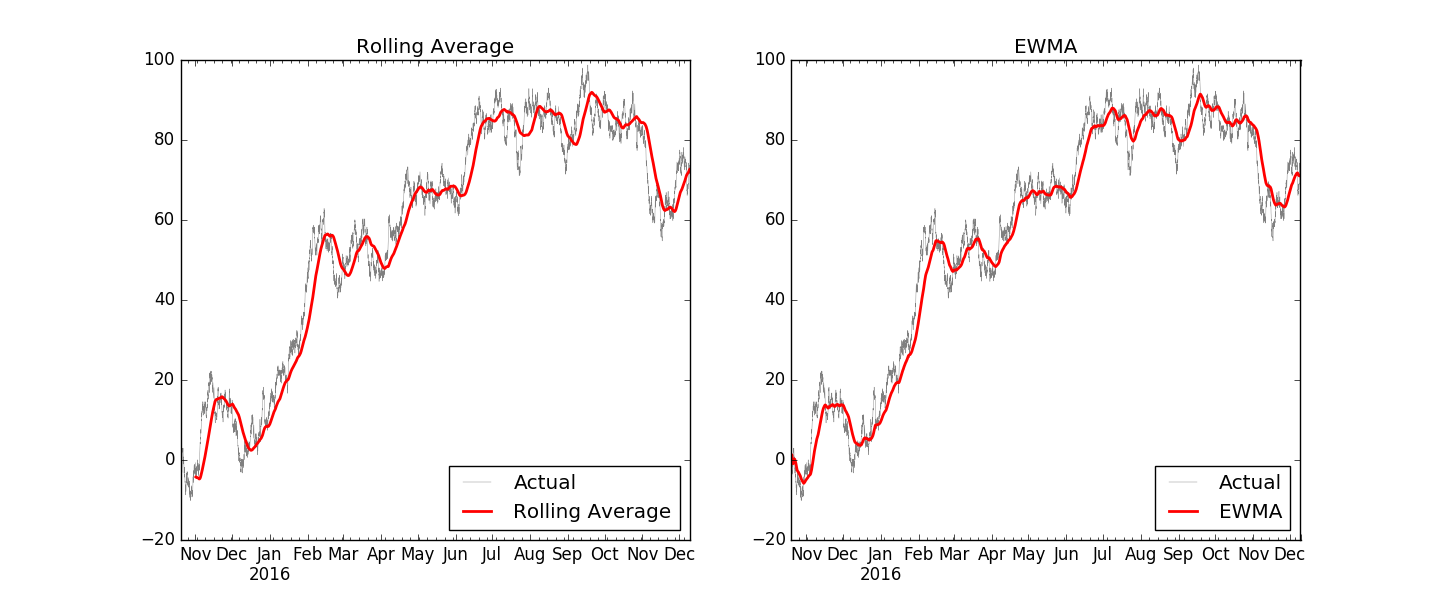
\includegraphics[width=\textwidth]{moving.png}
    \caption{Rolling average and EWMA}
\end{figure}

\begin{lstlisting}
s.plot(lw=.3, color='grey', label="Actual")
s.ewm(span=200).mean().plot(color='r', lw=2, label="EWMA")
plt.legend(loc="lower right")
plt.show()
\end{lstlisting}

\begin{problem} \label{prob:averages}
In this problem, we will explore the differences between rolling functions and EWM functions.

Generate a time series plot with the following information from the DJIA dataset:
    \begin{itemize}
        \item The original data points.
        \item Rolling average with window 30.
        \item Rolling average with window 365.
        \item Exponential average with span 30.
        \item Exponential average with span 365.
    \end{itemize}
Include a legend, axis labels, and title. Your plot should look like Figure \ref{fig:averages}.
\end{problem}

\begin{figure} \label{fig:averages}
    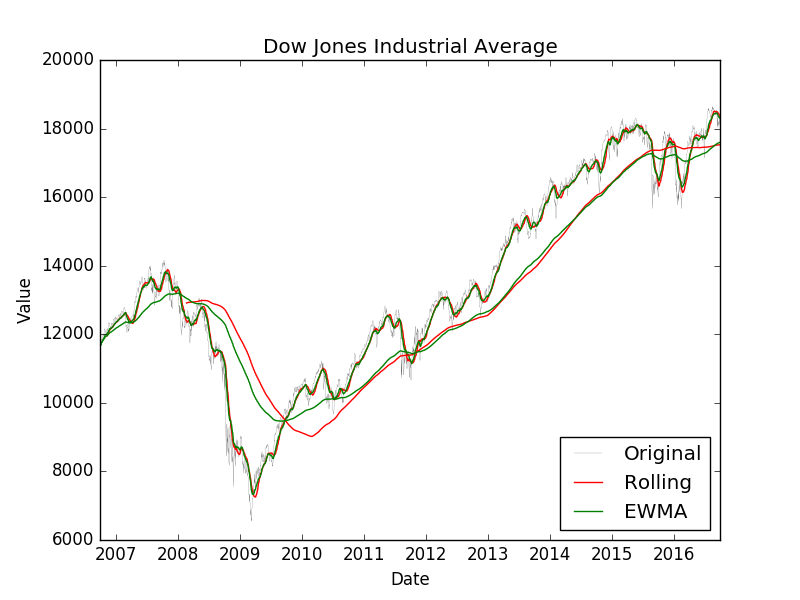
\includegraphics[width=\textwidth]{dow_averages.png}
    \caption{Rolling average and EWMA with windows 30 and 365.}
\end{figure}

\begin{problem} \label{prob:rolling_bound}
Plot the rolling minimum and rolling maximum values over the DJIA dataset with a window size of 30. This will create a moving bound for all the data that is easy to visualize.
\end{problem}
